%----------------------------------------------------------------------------------------
%	The Perceptron CHAPTER 
%----------------------------------------------------------------------------------------
\chapterimage{ChapterCover.pdf} % Chapter heading image
\chapter{Feature Processing in Visual Cortex}

\epigraph{\textit{The only thing worse than being blind is having sight but no vision.}}{\rightline{{\rm --- \href{https://www.womenshistory.org/education-resources/biographies/helen-keller}{Helen Keller}}}}

\minitoc
\newpage
\section{Introduction to Visual Feature Processing}
Feature detection in the visual system begins with specialized neural mechanisms that extract basic visual elements from incoming sensory information. These mechanisms operate through parallel processing channels that simultaneously analyze different aspects of the visual scene, including orientation, spatial frequency, motion, and contrast.

Visual processing begins at the retina, where specialized photoreceptors convert light into neural signals. This initial stage implements fundamental processing principles through center-surround receptive fields, which enhance local contrast detection. The retinal ganglion cells perform the first stage of feature extraction, responding selectively to differences in light intensity across their receptive fields.

From the retina, visual information travels through the lateral geniculate nucleus (LGN) to the primary visual cortex (V1), where more sophisticated feature detection begins. In V1, simple cells respond to oriented edges and lines at specific positions in their receptive fields, acting as basic feature detectors. These cells implement a form of spatial filtering, effectively decomposing the visual scene into its fundamental components of orientation and spatial frequency.
\begin{wrapfigure}{R}{0.6\textwidth}
\begin{tcolorbox}[every float=\centering, drop shadow, title=Organization of the Retina ,colback=white,colframe=WMgreen,
  colbacktitle=WMgreen,]
 \begin{tikzpicture}
  % Nodes for layers
  \node[draw, circle, fill=red!50] (P1) at (0, 4) {};
  \node[draw, circle, fill=red!50] (P2) at (1, 4) {};
  \node[draw, circle, fill=red!50] (P3) at (2, 4) {};
  \node[draw, circle, fill=red!50] (P4) at (3, 4) {};

  %\node[draw, circle, fill=green!50] (H1) at (0.5, 3) {};
  \node[draw, ellipse, minimum width=2cm, minimum height=.2cm, fill=green!50] (H1) at (.7,3) {};
  \node[draw, ellipse, minimum width=2cm, minimum height=.2cm, fill=green!50] (H2) at (2.3,3) {};
  %\node[draw, circle, fill=green!50] (H2) at (2.5, 3) {};

  \node[draw, circle, fill=blue!50] (B1) at (0.5, 2) {};
  \node[draw, circle, fill=blue!50] (B2) at (2.5, 2) {};

 \node[draw, ellipse, minimum width=2cm, minimum height=.2cm, fill=orange!50] (A1) at (.7,1) {};
  \node[draw, ellipse, minimum width=2cm, minimum height=.2cm, fill=orange!50] (A2) at (2.3,1) {};
 % \node[draw, circle, fill=orange!50] (A1) at (0, 1) {};
  %\node[draw, circle, fill=orange!50] (A2) at (1, 1) {};
  %\node[draw, circle, fill=orange!50] (A3) at (2, 1) {};
  %\node[draw, circle, fill=orange!50] (A4) at (3, 1) {};

  \node[draw, circle, fill=purple!50] (G1) at (1.5, 0) {};

  % Connections
  \foreach \i in {P1,P2,P3,P4} {
    \foreach \j in {H1,H2} {
      \draw[thin] (\i) -- (\j);
    }
  }

  \foreach \i in {H1,H2} {
    \foreach \j in {B1,B2} {
      \draw[thin] (\i) -- (\j);
    }
  }

  \foreach \i in {B1,B2} {
    \foreach \j in {A1,A2} {
      \draw[thin] (\i) -- (\j);
    }
  }

  \foreach \i in {A1,A2} {
    \draw[thin] (\i) -- (G1);
  }

  % Labels
  \node[align=left] at (5, 4) {\textbf{Photoreceptors}};
  \node[align=left] at (5, 3) {\textbf{Horizontal Cells}};
  \node[align=left] at (5, 2) {\textbf{Bipolar Cells}};
  \node[align=left] at (5, 1) {\textbf{Amacrine Cells}};
  \node[align=left] at (5, 0) {\textbf{Ganglion Cells}};
  \node[align=left] at (5, -1) {\textbf{Optic Nerve}};
  \node[align=left] at (5,-2) {\textbf{Receptive Field}};

  % Light rays
  \draw[blue, very thick, ->] (-1.5, 4) -- (-1.5, -2);
   \node[rotate=270, anchor=south] at (-1.5,1) {Signaling};
    %signaling
   \draw[yellow, very thick, ->] (-2, -2) -- (-2, 4);
   \node[rotate=90, anchor=north] at (-2.6,1) {Light};
  %\draw[yellow, very thick, ->] (-0.5, 5) -- (0, 4.5);
  %\draw[yellow, very thick, ->] (0, 5) -- (0.5, 4.5);

  %optic nerve
  \draw[black, very thick, ->] (1.5,0) -- (1.5, -1.5);
  
  %RF
  \node[draw, ellipse, minimum width=2.5cm, minimum height=.6cm, fill=blue!30] (rfsurround) at (1.5,-2) {};
    \node[draw, ellipse, minimum width=1.5cm, minimum height=.2cm, fill=blue] (rfcenter) at (1.5,-2) {};
\end{tikzpicture}
 \captionof{figure}{Organization of the cells of the retina.  Signaling initiated by the photoreceptors is filtered by a network of horizontal, bipolar, and amacrine cells as it is passed to the retinal ganglion cells, resulting in their center-surround receptive fields}
  \label{fig:retina}
 \end{tcolorbox}
 \end{wrapfigure}

As information flows through higher visual areas (V2, V3, V4, etc.), the processing becomes progressively more sophisticated. Simple cells in V1 converge onto complex cells that respond to oriented edges regardless of exact position, demonstrating how the system builds invariant representations. This hierarchical convergence continues through the ventral visual stream, where neurons become selective for increasingly complex features - from simple edges in V1, to contours and shapes in V2 and V3, to object parts in V4, and finally to whole objects in inferior temporal cortex. This organization reflects a fundamental principle of neural computation where simpler features are progressively combined to represent more complex visual attributes, allowing the brain to efficiently process and understand visual scenes.

\section{Retinal Filtering}
The retina plays a crucial role in the early stages of visual processing, performing complex computations on incoming visual information before it reaches the brain. This preprocessing in the retina allows for efficient and rapid analysis of visual scenes by extracting key features and distributing information across parallel channels.
\clearpage
\begin{wrapfigure}{R!}{0.4\textwidth}
\begin{tcolorbox}[every float=\centering, drop shadow, title=Mach Band Effect ,colback=white,colframe=WMgreen,
  colbacktitle=WMgreen,]
 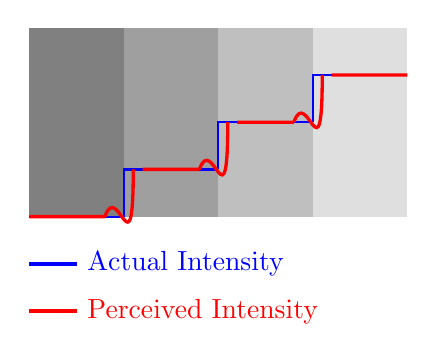
\begin{tikzpicture}[scale=1.2]
    % Create gradient bars with decreasing darkness (4 bars only)
    \foreach \x in {0,1,2,3} {
        \fill[gray!\the\numexpr 100-\x*25\relax] (\x,0) rectangle (\x+1,2);
    }
    
    % Draw actual intensity step function (directly over bars)
    \draw[thick, blue] (0,0) -- (1,0)
                 (1,0) -- (1,0.5) -- (2,0.5)
                 (2,0.5) -- (2,1.0) -- (3,1.0)
                 (3,1.0) -- (3,1.5) -- (4,1.5);
    
    % Draw perceived intensity with brief transitions (over bars)
    \draw[very thick, red] (0,0) -- (0.8,0)
                 (0.8,0) .. controls (0.94,0.4) and (1.1,-.65) .. (1.1,0.5)
                 (1.2,0.5) -- (1.8,0.5)
                 (1.8,0.5) .. controls (1.94,0.9) and (2.1,-0.15) .. (2.1,1.0)
                 (2.2,1.0) -- (2.8,1.0)
                 (2.8,1.0) .. controls (2.94,1.4) and (3.1,0.35) .. (3.1,1.5)
                 (3.2,1.5) -- (4,1.5);
    
    % Add labels
% Add legend below the bars
\draw[very thick, blue] (0,-0.5) -- (0.5,-0.5) node[right] {Actual Intensity};
\draw[very thick, red] (0,-1) -- (0.5,-1) node[right] {Perceived Intensity};
\end{tikzpicture}
 \captionof{figure}{Illustration of the Mach band effect.}
  \label{fig:MachBand}
 \end{tcolorbox}
 \end{wrapfigure}
 
The retina is composed of several layers of specialized neurons that work together to process visual input. When light enters the eye, it activates photoreceptors (rods and cones) in the outermost layer of the retina. These photoreceptors convert light into electrical signals, which are then passed through a network of bipolar cells, horizontal cells, amacrine cells, and ultimately to retinal ganglion cells (RGCs). Each of these cell types contributes to specific aspects of visual processing: Photoreceptors: Rods are responsible for scotopic (low-light) vision, while cones mediate photopic (bright-light) vision and color perception. Horizontal cells: These cells create lateral connections between photoreceptors and bipolar cells, enhancing contrast and sharpening edges in the visual scene. Bipolar cells: They relay signals from photoreceptors to RGCs, with some types responding to increases in light (ON bipolar cells) and others to decreases (OFF bipolar cells). Amacrine cells: These interneurons modulate the activity of bipolar cells and RGCs, contributing to motion detection and other complex visual features.
Retinal ganglion cells: RGCs are the output neurons of the retina, sending visual information to the brain via their axons, which form the optic nerve.
\begin{wrapfigure}{L!}{0.6\textwidth}
\begin{tcolorbox}[every float=\centering, drop shadow, title=Lateral Inhibition ,colback=white,colframe=WMgreen,
  colbacktitle=WMgreen,]
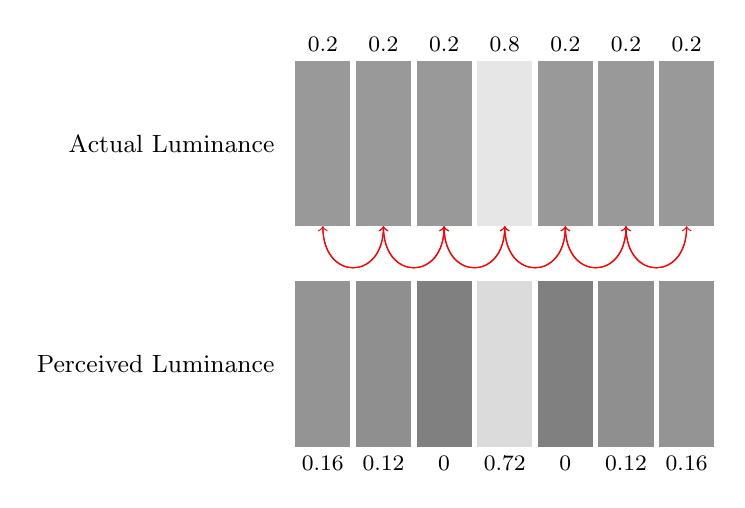
\begin{tikzpicture}[scale=.7]
    % Parameters
    \def\barwidth{1.0}
    \def\barheight{3.0}
    \def\spacing{0.1}

    % Luminance values
    \def\Lzero{0.2}
    \def\Lone{0.2}
    \def\Ltwo{0.2}
    \def\Lthree{.8}
    \def\Lfour{0.2}
    \def\Lfive{0.2}
    \def\Lsix{0.2}

    % Calculated perceived luminance
    \pgfmathsetmacro{\Pzero}{round((\Lzero - 0.2*(\Lone))*100)/100}
   \pgfmathsetmacro{\Pone}{round(max(\Lone - 0.2*(\Ltwo + \Lzero), 0)*100)/100}
    \pgfmathsetmacro{\Ptwo}{round(max(\Ltwo- 0.2*(\Lone + \Lthree), 0)*100)/100}
    \pgfmathsetmacro{\Pthree}{round((\Lthree - 0.2*(\Ltwo + \Lfour))*100)/100}
    \pgfmathsetmacro{\Pfour}{round(max(\Lfour - 0.2*(\Lthree + \Lfive), 0)*100)/100}
    \pgfmathsetmacro{\Pfive}{round(max(\Lfive - 0.2*(\Lfour + \Lsix), 0)*100)/100}
    \pgfmathsetmacro{\Psix}{round(max(\Lsix - 0.2*(\Lfive), 0)*100)/100}

    % Draw original luminance bars
    \foreach \i/\Lum in {0/\Lzero, 1/\Lone, 2/\Ltwo, 3/\Lthree, 4/\Lfour, 5/\Lfive, 6/\Lsix} {
        \pgfmathsetmacro{\grayvalue}{100-\Lum*100}
        \fill[gray!\grayvalue] (\i*\barwidth+\i*\spacing, 0) rectangle ++(\barwidth, \barheight);
        \node[above] at (\i*\barwidth+\i*\spacing+0.5*\barwidth, \barheight){\footnotesize{\pgfmathprintnumber[fixed, precision=1]{\Lum}}}; % {$\Lum$};
    }

    % Draw lateral inhibition curves
    \foreach \i in {0,...,5} {
        \pgfmathsetmacro{\startx}{\i*\barwidth+\i*\spacing+0.5*\barwidth}
        \pgfmathsetmacro{\endx}{(\i+1)*\barwidth+(\i+1)*\spacing+0.5*\barwidth}
        \draw[red, ->] (\startx, 0) .. controls (\startx, -1) and (\endx, -1) .. (\endx, 0);
        \draw[red, ->] (\endx, 0) .. controls (\endx, -1) and (\startx, -1) .. (\startx, 0);
    }

    % Draw perceived luminance bars
    \foreach \i/\Perc in {0/\Pzero, 1/\Pone, 2/\Ptwo, 3/\Pthree, 4/\Pfour, 5/\Pfive, 6/\Psix} {
        \pgfmathsetmacro{\grayvalue}{100-\Perc*100}
        \fill[gray!\grayvalue] (\i*\barwidth+\i*\spacing, -4) rectangle ++(\barwidth, \barheight);
        \node[below] at (\i*\barwidth+\i*\spacing+0.5*\barwidth, -4) {\footnotesize{\pgfmathprintnumber[fixed, precision=2]{\Perc}}}; %{$\Perc$};
    }

    % Labels
    \node[left] at (-.2, 1.5) {\small{Actual Luminance}};
    \node[left] at (-.2, -2.5) {\small{Perceived Luminance}};
    

    % Title
   % \node[above] at (3*\barwidth+3*\spacing, 4) {\textbf{Effect of Lateral Inhibition on Contrast}};
    
    % Mathematical model
    %\node[right] at (7.5, -1) {
     %   \begin{tabular}{l}
      %      \textbf{Mathematical Model:} \\
      %      $P_i = \max(L_i - k(L_{i-1} + L_{i+1}), 0)$ \\
        %    where: \\
          %  $P_i$: Perceived luminance \\
         %   $L_i$: Original luminance \\
           % $k$: Inhibition strength (0.1) \\
        %\end{tabular}
   % };
\end{tikzpicture}
 \captionof{figure}{\small{Illustration of how uniform lateral inhibition works to increase contrast at boundaries. This model assumes that the perceived luminance value in the receptive field for RGC $i$, $P_i$, is simply the actual luminance, $L_i$, minus the inhibition by its immediate neighbors, which is a proportion, $k$, of the their actual luminance. In other words, we use the actual luminance values to compute the perceived luminance for each of the RGCs pictured so that $P_i=L_i-k(L_i-1 + L_i+1)$.  The example illustrates the model with $k=2$.}}
  \label{fig:LatInhibition}
 \end{tcolorbox}
\end{wrapfigure}

One of the key functions of retinal processing is to perform early filtering of visual information. This filtering begins with the center-surround organization of RGC receptive fields. Each RGC responds most strongly to light hitting a small region in the center of its receptive field, with the surrounding area having an opposing effect. This organization allows for the detection of local contrast and edges through lateral inhibition, which enhances contrast sensitivity by suppressing uniform regions while amplifying differences at edges. This is evident in phenomena like the Mach band effect, where lateral inhibition creates exaggerated brightness transitions at edges.

Lateral inhibition in the retina creates the fundamental building blocks for visual processing through the establishment of center-surround receptive fields for the RGC. The center-surround organization of RGC receptive fields emerges through a complex interplay of neural circuits operating at multiple levels. Light information from photoreceptors first synapses onto ON and OFF bipolar cells, which respond oppositely to glutamate released by photoreceptors. ON bipolar cells are activated by light (inhibited by glutamate), while OFF bipolar cells are inhibited by light (excited by glutamate). These bipolar cells then connect to retinal ganglion cells in a parallel pathway, maintaining the ON/OFF organization. When light hits the center of a ganglion cell's receptive field, it can either excite the cell through ON bipolar cells or inhibit it through OFF bipolar cells, creating ON-center or OFF-center ganglion cells respectively. 
\begin{figure}[h!]
\begin{tcolorbox}[every float=\centering, drop shadow, title=Center-Surround Receptive Fields ,colback=white,colframe=WMgreen,
  colbacktitle=WMgreen,]
 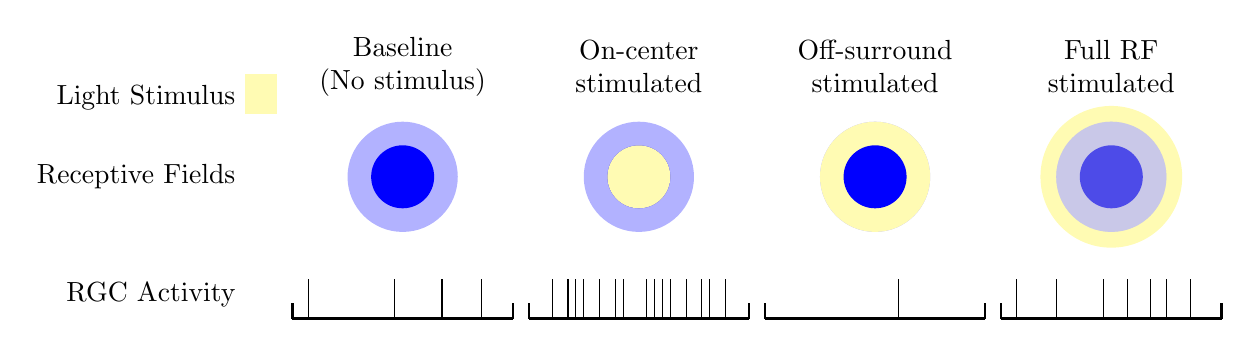
\begin{tikzpicture}
%Receptive Fields
  %whole RF
  \fill[yellow!30] (15,3) circle (.9);
  
\foreach \x in {6,9,12,15} {
        \fill[blue!30] (\x,3) circle (0.7);
        \fill[blue] (\x,3) circle (0.4);
    }
    \node [align=center] at (6,4.4) {Baseline \\ (No stimulus)};
     \node [align=center] at (9,4.4) {On-center \\ stimulated};
     \node [align=center] at (12,4.4) {Off-surround \\ stimulated};
     \node [align=center] at (15,4.4) {Full RF \\ stimulated};
  %Baseline activation
  \draw[thick] (4.6,1.2) -- (7.4,1.2);
  \draw[thick] (4.6,1.2) -- (4.6,1.4);
  \draw[thick] (7.4,1.2) -- (7.4,1.4);
  \draw[thin](4.8,1.2)--(4.8,1.7);
 % \draw[thin](5.3,1.2)--(5.3,1.7);
  \draw[thin](5.9,1.2)--(5.9,1.7);
  \draw[thin](6.5,1.2)--(6.5,1.7);
  \draw[thin](7,1.2)--(7,1.7);
  %On center
  \draw[thick] (7.6,1.2) -- (10.4,1.2);
  \draw[thick] (7.6,1.2) -- (7.6,1.4);
  \draw[thick] (10.4,1.2) -- (10.4,1.4);
  \draw[thin](9.4,1.2)--(9.4,1.7);
  \draw[thin](9.6,1.2)--(9.6,1.7);
  \draw[thin](7.9,1.2)--(7.9,1.7);
  \draw[thin](8.1,1.2)--(8.1,1.7);
  \draw[thin](8.2,1.2)--(8.2,1.7);
  \draw[thin](8.3,1.2)--(8.3,1.7);
  \draw[thin](8.5,1.2)--(8.5,1.7);
  \draw[thin](8.7,1.2)--(8.7,1.7);
  \draw[thin](8.8,1.2)--(8.8,1.7);
  \draw[thin](9.1,1.2)--(9.1,1.7);
  \draw[thin](9.2,1.2)--(9.2,1.7);
  \draw[thin](9.3,1.2)--(9.3,1.7);
  \draw[thin](9.8,1.2)--(9.8,1.7);
  \draw[thin](9.9,1.2)--(9.9,1.7);
  \draw[thin](10.1,1.2)--(10.1,1.7);
  %Off surround
  \draw[thick] (10.6,1.2) -- (13.4,1.2);
  \draw[thick] (10.6,1.2) -- (10.6,1.4);
  \draw[thick] (13.4,1.2) -- (13.4,1.4);
  \draw[thin](12.3,1.2)--(12.3,1.7);
  %full RF
  %Baseline activation
  \draw[thick] (13.6,1.2) -- (16.4,1.2);
  \draw[thick] (13.6,1.2) -- (13.6,1.4);
  \draw[thick] (16.4,1.2) -- (16.4,1.4);
  \draw[thin](13.8,1.2)--(13.8,1.7);
  \draw[thin](14.3,1.2)--(14.3,1.7);
  \draw[thin](14.9,1.2)--(14.9,1.7);
  \draw[thin](15.2,1.2)--(15.2,1.7);
  \draw[thin](15.5,1.2)--(15.5,1.7);
  \draw[thin](15.7,1.2)--(15.7,1.7);
  \draw[thin](16,1.2)--(16,1.7);
  %center fill
  \fill[yellow!30] (9,3) circle (0.4);
  %surround fill
  \fill[yellow!30] (12,3) circle (0.7);
  \fill[blue] (12,3) circle (0.4);
 %whole RF
 \fill[yellow!30, fill opacity=.3] (15,3) circle (.7);
  %Row labels
  \node[left] at (4,3) {Receptive Fields};
  \node[left] at (4,1.5) {RGC Activity};
 %legend
 \fill[yellow!30] (4,3.8) rectangle (4.4,4.3);
 \node[left] at (4,4) {Light Stimulus};
 \end{tikzpicture}
  \captionof{figure}{Responses by on-center retinal ganglion cells (RCGs) following various light stimuli.  The baseline represents the baseline firing rate of the RCG when no light stimulus is present.  the RCG is maximally activated when the light stimulus fall only on the on-center region of the RF.  Similarly, the RCG is maximally suppressed when only the off-surround is stimulated by light.  Finally, if the light stimulus covered both the on-center and off-surround, only a slight increase in activity from baseline may be observed.}
  \label{fig:OnCenterRFs}
 \end{tcolorbox}
\end{figure}
 
 In the outer retina, photoreceptors make excitatory connections to bipolar cells, creating the "center" response. These same photoreceptors also connect to horizontal cells, which spread the signal laterally and provide inhibitory feedback to neighboring photoreceptors. This horizontal cell feedback creates an initial antagonistic surround effect, where stimulation of the surrounding area produces the opposite response to stimulation of the center. The inner retina adds another layer of lateral inhibition through amacrine cells, which further refine the center-surround organization. The system effectively compares the light falling on one area of the retina with the light falling on adjacent areas, making cells particularly responsive to differences in illumination between the center and surround regions.

These ON and OFF pathways remain segregated as the information travels through the lateral geniculate nucleus (LGN) to V1, where multiple center-surround units are combined to create more complex receptive fields like edge detectors. The parallel processing of ON and OFF information allows the visual system to efficiently encode both light increments and decrements. The retina also performs parallel processing of different visual properties. Different types of RGCs extract specific features from the visual scene, such as luminance, local contrast, spatial and temporal frequency, motion, motion direction, and color. This parallel processing enables the brain to analyze visual information rapidly and efficiently based on these pre-extracted features.

By performing these complex computations and filtering operations, the retina significantly reduces the amount of raw visual data that needs to be transmitted to and processed by the brain. This preprocessing allows higher-level visual areas to focus on more complex tasks such as object recognition, motion analysis, and scene interpretation.

\section{Simple Cells \& Orientation Selectivity}
Simple cells in the primary visual cortex (V1) play a crucial role in early visual processing, particularly in orientation selectivity and edge detection. These neurons, first described by David Hubel and Torsten Wiesel, have elongated receptive fields with distinct excitatory and inhibitory regions arranged in parallel12. This unique structure allows simple cells to respond selectively to oriented stimuli, such as bars or edges with specific orientations in their receptive fields.

The orientation selectivity of simple cells arises from the convergence of inputs from lateral geniculate nucleus (LGN) cells. According to Hubel and Wiesel's model, several LGN cells with center-surround receptive fields are arranged in a line, forming the elongated structure of a simple cell's receptive field2. This arrangement results in a narrow receptive field for the simple cell, with its preferred orientation aligned with the arrangement of LGN inputs1.
\begin{wrapfigure}{L!}{0.4\textwidth}
\begin{tcolorbox}[every float=\centering, drop shadow, title=Simple Cells in V1 ,colback=white,colframe=WMgreen,
  colbacktitle=WMgreen,]

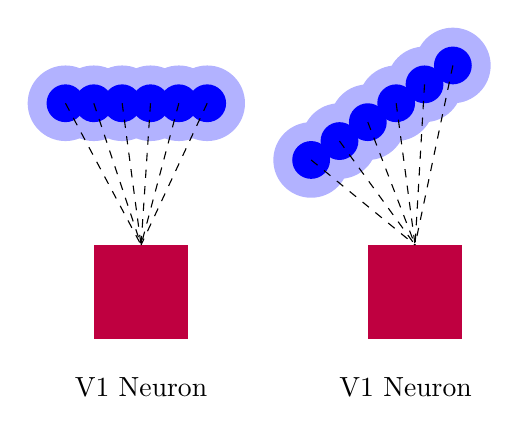
\begin{tikzpicture}[scale=1.2]
    
    % Part B: V1 Integration
    % Title for Part B
    % Center-surround receptive fields
    \foreach \x in {-.8,-.5,-.2,.1,.4,.7} {
        \fill[blue!30] (\x,3) circle (0.4);
    }
    \foreach \x in {-.8,-.5,-.2,.1,.4,.7}{
       \fill[blue] (\x,3) circle (0.2);
    }
   % \node at (7,3.5) {Center-Surround Fields}; 
    % V1 neuron
    \fill[purple] (-.5,.5) rectangle (.5,1.5);
    \node at (0,0) {V1 Neuron};
    
    % Connections to V1
    \foreach \x in {-.8,-.5,-.2,.1,.4,.7} {
        \draw[dashed] (\x,3) -- (0,1.5);
    }
    
    %start of angle v1
     \foreach \x/\y in {1.8/2.4,2.1/2.6,2.4/2.8,2.7/3,3/3.2,3.3/3.4} {
        \fill[blue!30] (\x,\y) circle (0.4);
    }
     \foreach \x/\y in  {1.8/2.4,2.1/2.6,2.4/2.8,2.7/3,3/3.2,3.3/3.4} {
       \fill[blue] (\x,\y) circle (0.2);
    }
   % \node at (7,3.5) {Center-Surround Fields}; 
    % V1 neuron
    \fill[purple] (2.4,.5) rectangle (3.4,1.5);
    \node at (2.8,0) {V1 Neuron};
    
    % Connections to V1
    \foreach \x/\y in  {1.8/2.4,2.1/2.6,2.4/2.8,2.7/3,3/3.2,3.3/3.4} {
        \draw[dashed] (\x,\y) -- (2.9,1.5);
    }
\end{tikzpicture}
  \captionof{figure}{Illustration of how the convergence of RGC receptive fields on V1 neurons can produce edge detectors.}
  \label{fig:SimpleCells}
 \end{tcolorbox}
\end{wrapfigure}

Simple cells play a crucial role in spatial frequency analysis of visual information. These neurons, first described by Hubel and Wiesel, have elongated receptive fields with distinct excitatory and inhibitory regions arranged in parallel. This unique structure allows simple cells to act as spatial frequency filters, responding selectively to specific spatial frequencies in their receptive fields. 

Spatial frequency is a fundamental concept in visual perception and image processing that describes how rapidly brightness or color changes across space in an image or visual scene. It is typically measured in cycles per degree of visual angle or cycles per unit distance (e.g., cycles per millimeter).

The spatial frequency selectivity of simple cells arises from the organization of their receptive fields. The width of the excitatory and inhibitory subregions in a simple cell's receptive field corresponds closely to the spatial frequency to which the cell responds most strongly1. This relationship between receptive field structure and spatial frequency tuning suggests that simple cells perform a local Fourier analysis of the visual scene.

Simple cells exhibit a range of preferred spatial frequencies, typically spanning from 0.2 to 2.0 cycles per degree in cats8. This diversity allows the visual system to analyze different scales of spatial information in parallel. Importantly, the spatial frequency selectivity of simple cells is often sharper than that of their inputs from the lateral geniculate nucleus (LGN), indicating that cortical mechanisms enhance and refine spatial frequency tuning4.

The responses of simple cells to sinusoidal gratings can be predicted remarkably well from their spatial receptive fields2. This quasi-linear behavior extends to more complex stimuli, including natural scenes. However, there is evidence of nonlinear mechanisms that further shape spatial frequency selectivity, particularly in the suppression of responses to non-preferred spatial frequencies.

\begin{wrapfigure}{R!}{0.5\textwidth}
\begin{tcolorbox}[every float=\centering, drop shadow, title=Concept of Spatial Frequency ,colback=white,colframe=WMgreen,
  colbacktitle=WMgreen,]
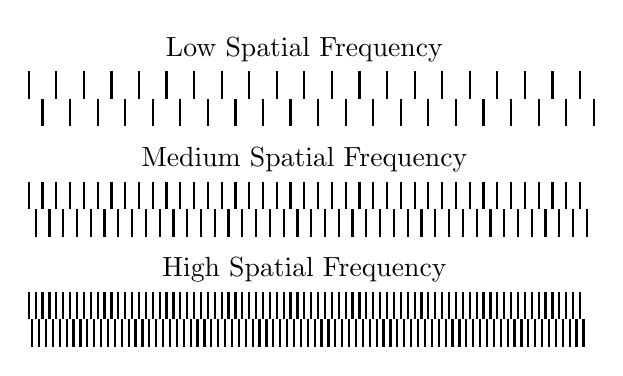
\begin{tikzpicture}[scale=.7]

% Low spatial frequency sinusoidal pattern
\foreach \x in {0, 0.5, ..., 10} {
    \draw[thick] (\x, 4) -- ++(0, 0.5);
    \draw[thick] (\x+0.25, 4) -- ++(0, -0.5);
}
\node[above] at (5, 4.5) {Low Spatial Frequency};

% Medium spatial frequency sinusoidal pattern
\foreach \x in {0, 0.25, ..., 10} {
    \draw[thick] (\x, 2) -- ++(0, 0.5);
    \draw[thick] (\x+0.125, 2) -- ++(0, -0.5);
}
\node[above] at (5, 2.5) {Medium Spatial Frequency};

% High spatial frequency sinusoidal pattern
\foreach \x in {0, 0.125, ..., 10} {
    \draw[thick] (\x, 0) -- ++(0, 0.5);
    \draw[thick] (\x+0.0625, 0) -- ++(0, -0.5);
}
\node[above] at (5, 0.5) {High Spatial Frequency};

\end{tikzpicture}
 \captionof{figure}{Illustration of stimuli with low, medium, and high spatial frequency.}
  \label{fig:spatialfrequency}
 \end{tcolorbox}
\end{wrapfigure}
\FloatBarrier

Interestingly, adjacent simple cells in V1 often have similar spatial frequency and orientation preferences but differ in their spatial phase. This arrangement suggests that groups of simple cells may function as quadrature pairs, effectively implementing sine and cosine filters for a given spatial frequency and orientation7. Such an organization would allow the visual system to encode both the magnitude and phase of spatial frequency components in the visual scene.

The spatial frequency analysis performed by simple cells contributes to various aspects of visual processing, including edge detection, texture analysis, and the initial stages of object recognition. By decomposing the visual scene into its constituent spatial frequencies, simple cells provide a foundation for more complex visual computations in higher cortical areas.

\section{Gabor Filters}
Gabor filters are powerful tools in image processing and computer vision, serving as spatial filters that can extract important features from images. Named after Dennis Gabor, these filters are particularly effective at analyzing textures, detecting edges, and extracting features that are, not unlike simple cells in V1, sensitive to both frequency and orientation information in images.

The Gabor filter is essentially a Gaussian kernel function modulated by a sinusoidal plane wave. In the spatial domain, it can be represented mathematically as: $G(x,y)=\exp{-\frac{x^2+y^2}{2}}\cdot cos(2\pi x)$.

Gabor filters are particularly useful because they can capture local spatial and frequency information simultaneously. This property makes them well-suited for texture analysis, edge detection, and feature extraction in various computer vision applications.

\begin{wrapfigure}{L}{0.4\textwidth}
\begin{tcolorbox}[every float=\centering, drop shadow, title=The Gabor Kernel Function ,colback=white,colframe=WMgreen,
  colbacktitle=WMgreen,]
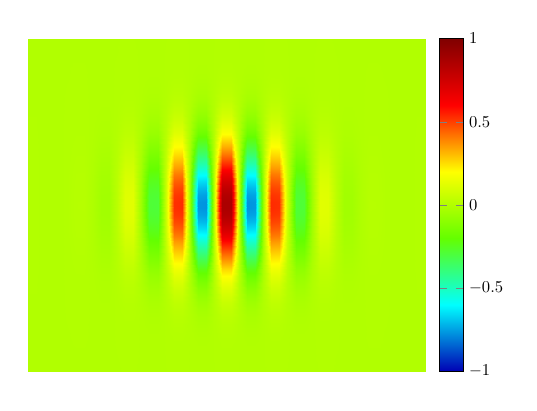
\begin{tikzpicture}[scale=.6]
    \begin{axis}[
        axis lines=none, % Simplifies the plot by removing axis lines
        width=10cm, % Sets the width of the plot
        domain=-4:4, % Range for x
        y domain=-4:4, % Range for y
        samples=50, % Number of samples for x
        samples y=50, % Number of samples for y
        colormap/bluered, % Color scheme: blue (small) to red (large)
        view={0}{90}, % Top-down 2D view
        colorbar, % Adds a colorbar for intensity scale
        point meta min=-1, % Minimum value for color scaling
        point meta max=1 % Maximum value for color scaling
    ]
        % Gabor kernel equation
        \addplot3[
            surf,
            shader=interp % Smooth interpolation for surface
        ]
        {exp(-0.5*(x^2 + y^2)) * cos(deg(2*3.14159*x))};
    \end{axis}
\end{tikzpicture}
 \captionof{figure}{2-dimensional Illustration of a Gabor kernel.}
  \label{fig:gabor}
 \end{tcolorbox}
\end{wrapfigure}
\FloatBarrier

One of the key advantages of Gabor filters is their similarity to the human visual system's processing of visual information. The filters' frequency and orientation representations are similar to those of the human visual cortex, making them biologically inspired and effective for mimicking human perception in computer vision tasks35. By varying parameters such as frequency, orientation, and bandwidth, we can create a bank of Gabor filters that can extract a rich set of features from an image.

When applied to an image through convolution, Gabor filters can highlight different texture characteristics and orientations. For example, by using Gabor filters with different orientations, we can detect edges and lines in various directions within an image. Similarly, by adjusting the frequency parameter, we can extract features at different scales, allowing for the analysis of both fine and coarse textures. The features extracted using Gabor filters can be used in various machine learning tasks, such as texture classification, object recognition, and image segmentation. 

Convolution is a fundamental operation in image processing and computer vision that involves sliding a small matrix, called a kernel or filter, over an input image to produce a new output image. The process works by multiplying each pixel in the input image by the corresponding value in the kernel, summing the results, and placing this sum in the corresponding position of the output image. This operation allows for various image transformations, including blurring, sharpening, and edge detection, depending on the values in the kernel.

\begin{figure}[h!]
\centering
\begin{tcolorbox}[every float=\centering, drop shadow, title=Image Filtering by Convolution ,colback=white,colframe=WMgreen,
  colbacktitle=WMgreen,]
  \centering
\begin{tikzpicture}[
    2d-arr/.style={matrix of nodes, row sep=-\pgflinewidth, column sep=-\pgflinewidth, nodes={draw, minimum size=0.6cm}},
    pixel/.style={fill=black!#1, text=blue}
]

% Input image (letter T)
\matrix (input) [2d-arr] {
    |[pixel=0]| 0 & |[pixel=0]| 0 & |[pixel=0]| 0 & |[pixel=60]| 1 & |[pixel=0]| 0 & |[pixel=0]| 0 & |[pixel=0]| 0\\
    |[pixel=0]| 0 & |[pixel=0]| 0 & |[pixel=0]| 0 & |[pixel=60]| 1 & |[pixel=0]| 0 & |[pixel=0]| 0 & |[pixel=0]| 0\\
    |[pixel=60]| 1 & |[pixel=60]| 1 & |[pixel=60]| 1 & |[pixel=60]| 1 & |[pixel=60]| 1 & |[pixel=60]| 1 & |[pixel=60]| 1\\
    |[pixel=0]| 0 & |[pixel=0]| 0 & |[pixel=0]| 0 & |[pixel=60]| 1 & |[pixel=0]| 0 & |[pixel=0]| 0 & |[pixel=0]| 0\\
    |[pixel=0]| 0 & |[pixel=0]| 0 & |[pixel=0]| 0 & |[pixel=60]| 1 & |[pixel=0]| 0 & |[pixel=0]| 0 & |[pixel=0]| 0\\
    |[pixel=0]| 0 & |[pixel=0]| 0 & |[pixel=0]| 0 & |[pixel=60]| 1 & |[pixel=0]| 0 & |[pixel=0]| 0 & |[pixel=0]| 0\\
    |[pixel=0]| 0 & |[pixel=0]| 0 & |[pixel=0]| 0 & |[pixel=60]| 1 & |[pixel=0]| 0 & |[pixel=0]| 0 & |[pixel=0]| 0\\
};
\node[below=of input-6-4] {Input Image};

% Convolution operator
\node[right=0.5cm of input] (conv) {$*$};

% Kernel (edge detection)
\matrix (kernel) [2d-arr, right=0.5cm of conv, nodes={draw, minimum size=0.5cm}] {
    |[pixel=0]| 0 & |[pixel=50]| .5 & |[pixel=0]| 0 \\
    |[pixel=0]| 0 & |[pixel=750]| 1 & |[pixel=0]| 0 \\
    |[pixel=0]| 0 & |[pixel=50]| .5 & |[pixel=0]| 0 \\
};
\node[below=0.5cm of kernel-3-2] {Kernel};

% Equals sign
\node[right=0.5cm of kernel] (eq) {$=$};

% Output (edge-detected T)
\matrix (output) [2d-arr, right=0.5cm of eq] {
    |[pixel=25]| .5 & |[pixel=25]| .5 & |[pixel=100]| 2 & |[pixel=25]| .5 & |[pixel=25]| .5\\
    |[pixel=60]| 1 & |[pixel=60]| 1 & |[pixel=100]| 2 & |[pixel=60]| 1 & |[pixel=60]| 1 \\
    |[pixel=25]| .5 & |[pixel=25]| .5 & |[pixel=100]| 2 & |[pixel=25]| .5 & |[pixel=25]| .5\\
    |[pixel=0]| 0 & |[pixel=0]| 0 & |[pixel=100]| 2 & |[pixel=0]| 0 & |[pixel=0]| 0 \\
    |[pixel=0]| 0 & |[pixel=0]| 0 & |[pixel=100]| 2 & |[pixel=0]| 0 & |[pixel=0]| 0\\
};
\node[below=of output-4-3] {Output};

% Highlight convolution area
\draw[dashed, red, very thick] (input-2-3.north west) rectangle (input-4-5.south east);
\draw[dashed, blue, very thick] (output-2-3.north west) rectangle (output-2-3.south east);
\draw[<-, red, thick] (kernel-2-1) to[bend left] (input-4-5);
\draw[->, blue, thick] (kernel-2-3) to[bend right] (output-2-3);

\end{tikzpicture}
 \captionof{figure}{Illustration of the convolution operation.  Here an input image with various luminance values is filtered using a simple gabor-like kernel.  Notice how convolution with a vertically oriented gabor kernel nicely exaggerates the vertical edges, but not the horizontal edges.}
  \label{fig:convolution}
 \end{tcolorbox}
\end{figure}
\FloatBarrier

The convolution operation is particularly powerful because it can extract meaningful features from images. By using different kernels, we can emphasize various aspects of an image, such as edges, textures, or specific patterns. One type of filter that leverages convolution for feature analysis is the Gabor filter.

Research has shown that Gabor filters provide a reasonably accurate description of most spatial aspects of simple receptive fields in V1. Simple cells in the visual cortex exhibit responses that can be well-modeled by Gabor-like functions, with specific orientations, spatial frequencies, and phases1. This correspondence suggests that the visual system has evolved to efficiently extract relevant features from visual stimuli, much like Gabor filters do in image processing applications. The Gabor function's ability to simultaneously represent information in both spatial and frequency domains aligns with the visual system's need to analyze both local and global image properties2.

\begin{figure}[h!]
\centering
\begin{tcolorbox}[every float=\centering, drop shadow, title=Varying Orientation and Wavelength of the Gabor Filters ,colback=white,colframe=WMgreen,
  colbacktitle=WMgreen,]
  \centering
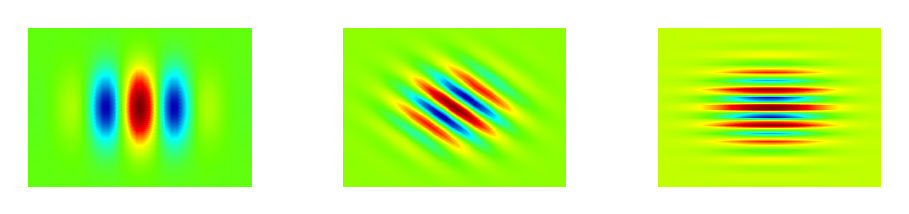
\begin{tikzpicture}[scale=2]
    \foreach \freq/\angle in {0.5/0, 1.0/45, 1.5/90}{
        \begin{scope}[shift={(\freq*4cm,0)}]
            \begin{axis}[
                axis lines=none,
                width=3cm,
                domain=-3:3,
                y domain=-3:3,
                samples=40,
                samples y=40,
                colormap/bluered,
                view={0}{90}
            ]
                \addplot3[surf, shader=interp]
                {exp(-0.5*(x^2 + y^2)) * 
                 cos(deg(2*pi*(\freq*(x*cos(\angle) + y*sin(\angle)))))};
            \end{axis}
        \end{scope}
    }
\end{tikzpicture}
 \captionof{figure}{Illustration of various gabor filters with decreasing wavelength ($\lambda$) and increasing angle of rotation from left to right.}
  \label{fig:gaborangles}
 \end{tcolorbox}
\end{figure}
\FloatBarrier

However, it's important to note that while Gabor filters provide a good approximation of simple cell responses, they do not capture the full complexity of neural processing in V1. Recent studies using convolutional neural networks (CNNs) have suggested that V1 neurons may involve more nonlinear computations than previously thought. Nonetheless, even in these more complex models, Gabor-like filters often emerge in the early layers, indicating their fundamental importance in visual processing. The relationship between Gabor filters and neural responses underscores the biological inspiration behind many computer vision algorithms and highlights the efficiency of the visual system in extracting meaningful information from the environment.

The output from convolving an image with a Gabor filter provides valuable information about the texture and edge characteristics of the image at specific orientations and frequencies. Here's how to interpret this output:

\begin{itemize}
    \item Magnitude Response
The magnitude of the Gabor filter output indicates the strength of the texture or edge features in the image that match the filter's parameters:
High magnitude values correspond to areas in the image where there is a strong presence of features (such as edges or textures) that align with the filter's orientation and frequency. Low magnitude values indicate regions where such features are absent or weak.
    \item Interpretation Based on Filter Parameters
The interpretation of the output depends on the specific parameters of the Gabor filter used:

Orientation ($\theta$): The output will highlight features oriented in the direction specified by $\theta$. For example, a filter with $\theta = 0\deg$ will respond strongly to horizontal features.

Wavelength ($\lambda$): This parameter determines the scale of features detected. Smaller wavelengths detect finer textures, while larger wavelengths capture coarser structures2.

Bandwidth ($\sigma$): This affects the range of frequencies the filter responds to. A larger $\sigma$ results in a broader response to a range of frequencies.

    \item Multiple Filter Responses
Often, a bank of Gabor filters with different orientations and scales is used:
By analyzing the responses across multiple filters, you can build a comprehensive representation of the image's texture and edge characteristics.
\end{itemize}

\printglossary[type=datacollection,style=twocolumn]
%\printglossary
%\glsresetall
\newpage
\bibliographystyle{apalike}
\renewcommand{\bibname}{References}
\bibliography{bibliography}
